\documentclass[usenames,dvipsnames]{beamer}

\usepackage{tikz}
\usepackage{tkz-berge}
\usepackage{tkz-graph}

\usetikzlibrary{patterns,arrows,decorations.pathreplacing}

\usepackage{xcolor}
\definecolor{dblue}{RGB}{20,66,129}
\definecolor{rose}{RGB}{255,101,122}
\definecolor{crimsonred}{RGB}{132,22,23}

\definecolor{olive}{rgb}{0.3, 0.4, .1}
\definecolor{fore}{RGB}{249,242,215}
\definecolor{back}{RGB}{51,51,51}
\definecolor{title}{RGB}{255,0,90}
\definecolor{dgreen}{rgb}{0.,0.6,0.}
\definecolor{gold}{rgb}{1.,0.84,0.}
\definecolor{JungleGreen}{cmyk}{0.99,0,0.52,0}
\definecolor{BlueGreen}{cmyk}{0.85,0,0.33,0}
\definecolor{RawSienna}{cmyk}{0,0.72,1,0.45}
\definecolor{Magenta}{cmyk}{0,1,0,0}


\title{Fractals avoiding Fractal Sets}
\author{Jacob Denson}
\institute{University of British Columbia}

\begin{document}

\maketitle

\begin{frame}
  \frametitle{Pattern Avoidance Problems}

\begin{tabular}{p{0.8\textwidth}p{0.3\textwidth}}

\begin{itemize}
     \item How large can the Hausdorff dimension of a subset of $\mathbf{R}$ be not containing 3 term arithmetic progressions?

     %\pause
     \item What is the largest Hausdorff dimension of a subset of $\mathbf{R}^d$ such that the distances between any two points are distinct?

     %\pause
     \item What is the largest Hausdorff dimension of $\mathbf{R}^d$ such that the angles formed from any three points are irrational?
\end{itemize}

\end{tabular}

\end{frame}

\begin{frame}
    \frametitle{Two Observations}

    \begin{itemize}
        \item Problems can be summarized as finding $X$ such that $X^n$ avoids a given set $Z$, except for `repeated coordinate points'. Let
        \[ \Delta = \{ x \in (\mathbf{R}^d)^n: x_i = x_j\ \text{for distinct}\ i,j \in \{ 1, \dots, n \} \} \]
        %
        \vspace{-1.5em}

%            \begin{center}
%        \begin{tabular}{| c | c |}
%            \hline
%            $Z$ & Pattern Problem\\
%            \hline
%            $\{ (x,y,z) \in \mathbf{R}^3: z - x = 2(y-x) \}$ & $X^3 \cap Z \subset \Delta$ iff $X$ avoids three term arithmetic progressions.\\
%            $\{ (x,y,z,w) \in \mathbf{R}^{4d}: d(x,y) = d(z,w) \}$ & $X^4 \cap Z \subset \Delta$ if and only if the points in $X$ have distinct distances.\\
%            $\{ (x,y,z) \in \mathbf{R}^{3d}: \frac{(x - z) \cdot (y - z)}{|x-z||y-z|} = \cos(120^\circ) \}$ & $X^4 \cap Z \subset \Delta$ if and only if $X$ avoids $120^\circ$ angles.\\
%            \hline
%        \end{tabular}
%        \end{center}

        \begin{itemize}
           \item If $Z = \{ (x,y,z) \in \mathbf{R}^3: z - x = 2(y - x) \}$, $X$ avoids 3 term arithmetic progressions if and only if $X^3 \cap Z \subset \Delta$.

            \item If $Z = \{ (x,y,z,w): d(x,y) = d(z,w) \} \subset \mathbf{R}^{4d}$, then points in $X$ have distinct distances if and only if $X^4 \cap Z \subset \Delta$.

            \item If $Z = \{ (x,y,z): \frac{(x-z) \cdot (y-z)}{|x-z||y-z|} = \cos(120^\circ)\}$, $X$ avoids $120^\circ$ angles if and only if $X^3 \cap Z \subset \Delta$.
        \end{itemize}
    \end{itemize}
\end{frame}

\begin{frame}
    \frametitle{The Generic Problem}

    \begin{itemize}
        \item {\bf Fractal Avoidance Problem}: Given $Z \subset \mathbf{R}^{nd}$, find $X \subset \mathbf{R}^d$ with large Hausdorff dimension such that $X^n \cap Z \subset \Delta$.
        %\pause

        \item Math\'{e} (2012): If $Z$ is an algebraic hypersurface specified by a degree $r$ polynomial in $nd$ variables with rational coefficients, then we can find $X$ solving the fractal avoidance problem for $Z$ with dimension $d/r$. This is independent of $n$.
        %\pause

        \item Pramanik and Fraser (2016): If $Z$ is a smooth hypersurface of dimension $nd - d$, we can find $X$ with dimension $d/(n-1)$.
    \end{itemize}
\end{frame}

\begin{frame}
    \frametitle{Increasing the Difficulty$\dots$}

    \begin{center}
     \Huge {\it What if the Patterns are Fractally Specified...}
    \end{center}
\end{frame}

%\begin{frame}
%    \frametitle{The Avoidance Problem}

%        \begin{itemize}

%            \item Our method naturally considers an equivalent setup.

%            \item {\bf Fractal Avoidance Problem}: Given $Y \subset \mathbf{R}^{nd}$, find $X \subset \mathbf{R}^d$ such that $X^n \cap Y \subset \Delta$, where $\Delta = \{ x: x_i = x_j\ \text{for some $i,j$} \}$.

%            \item Equivalent by setting $Y = f^{-1}(0)$, or $f = \mathbf{I}_{Y^c}$.

%            \item Our method only uses the structure of the zero set, not $f$.
%        \end{itemize}
%\end{frame}

\begin{frame}
    \frametitle{Main Result}

    \begin{theorem}
        If $Z$ is the countable union of sets with lower Minkowski dimension bounded by $\alpha$, we can find $X$ with $X^n \cap Z \subset \Delta$ and
        %
        \[ \dim_{\mathbf{H}}(X) = \min \left( \frac{nd - \alpha}{n - 1}, d \right) = \min\left( \frac{\text{codim}(Z)}{n - 1}, 1 \right) \]
    \end{theorem}
    % Introduce Fractal Avoidance Problem

    %\pause

    \begin{itemize}
        \item Pramanik and Fraser's Result is a special case. Shows smoothness is only required to get a bound on the Hausdorff dimension.
    \end{itemize}
\end{frame}

\begin{frame}
    \frametitle{Low Rank Avoidance}

    \begin{theorem}
        If $Z$ is the countable union of sets $Z_i$ for which there exists a linear transformation $T_i: \mathbf{R}^{nd} \to \mathbf{R}^{kd}$, with rational coordinates such that $T_i(Z_i)$ has Minkowski dimension $\beta$ for each $i$, we can find $X$ with $X^n \cap Z \subset \Delta$ and
        %
        \[ \dim_{\mathbf{H}}(X) = \frac{nk - \beta}{2k - 1} = \frac{\text{codim}(T(Z))}{2k - 1} \]
    \end{theorem}

    %\pause
    \begin{itemize}
        \item You can think of the hypothesis as saying $Z$ is coverable efficiently by lower dimensional thickened hyperplanes in countably many directions. Result also extends to $Z$ which is efficiently covered by algebraic hypersurfaces.

        %\pause
        \item Really want to push the $2k - 1$ to $k - 1$, at least for $k \geq 2$. Know this is true for a large number of examples.
    \end{itemize}
\end{frame}

\begin{frame}
    \frametitle{Applications}

    \begin{center}
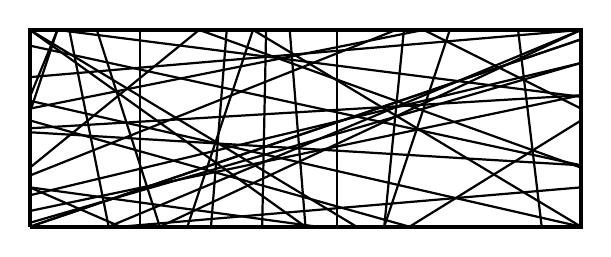
\begin{tikzpicture}[scale=0.5]
%\draw[help lines] (0,0) grid (14,5);

\draw[ultra thick] (0,0) -- (14,0) -- (14,5) -- (0,5) -- (0,0);

\draw[thick] (0,3.3) -- (0.7,5);
\draw[thick] (0,2.7) -- (9.642,0);
\draw[thick] (0,2.5) -- (14,3.34);
\draw[thick] (0,2.4) -- (14,1.56);
\draw[thick] (0,1) -- (2.3,0);
\draw[thick] (0,0) -- (14,4.76);
\draw[thick] (0,0.8) -- (14,4.16);
\draw[thick] (2.8,0) -- (2.8,5);
\draw[thick] (1.7,5) -- (3.3,0);
\draw[thick] (0,1.5) -- (4.3,5);
\draw[thick] (0,3) -- (10,5);
\draw[thick] (4,0) -- (5.66666,5);
\draw[thick] (1,5) -- (2,0);

\draw[thick] (0,2.9) -- (0.7,5);
\draw[thick] (0,3.2) -- (14,0);
\draw[thick] (0,0.4) -- (14,3.34);
\draw[thick] (0,4.6) -- (14,1.56);
\draw[thick] (0,1) -- (7.3,0);
\draw[thick] (0,0) -- (14,4.76);
\draw[thick] (0,0.1) -- (14,4.16);
\draw[thick] (7.8,0) -- (7.8,5);
\draw[thick] (0,5) -- (8.3,0);
\draw[thick] (0,1.3) -- (9.3,5);
\draw[thick] (0,3.8) -- (14,5);
\draw[thick] (9,0) -- (10.66666,5);
\draw[thick] (0,5) -- (7,0);

\draw[thick] (14,3.3) -- (0.7,5);
\draw[thick] (14,2.7) -- (9.642,0);
\draw[thick] (14,2.5) -- (14,3.34);
\draw[thick] (14,2.4) -- (14,1.56);
\draw[thick] (14,1) -- (2.3,0);
\draw[thick] (14,0) -- (14,4.76);
\draw[thick] (14,0.8) -- (14,4.16);
\draw[thick] (14,5) -- (3.3,0);
\draw[thick] (14,1.5) -- (4.3,5);
\draw[thick] (14,3) -- (10,5);
\draw[thick] (14,0) -- (5.66666,5);
\draw[thick] (14,5) -- (2,0);

\draw[thick] (7,0) -- (6.6,5);
\draw[thick] (9,0) -- (9.5,5);
\draw[thick] (13,0) -- (12.4,5);
\draw[thick] (4.6,0) -- (5,5);
\draw[thick] (5.9,0) -- (6,5);
\end{tikzpicture}
\end{center}

    \begin{itemize}
        \item More robust result of Pramanik and Fraser, showing that we can `thicken' or `thin' the zero set of our function with stable effects on the Hausdorff dimension of $X$.
        %\pause

        \item Uncountable unions of regular sets are allowed!
    \end{itemize}
\end{frame}

\begin{frame}
    \frametitle{Applications}

    \begin{itemize}
        \item Given a subset $Y$ of $\mathbf{R}^d$ which is the countable union of sets with Minkowski dimension $\alpha$, we can find a $\mathbf{Q}$ vector subspace $X$ of $\mathbf{R}^d$ with Hausdorff dimension $d - \alpha$ disjoint from $Y$.

        %\pause
        \item We can find a full dimensional subset of $\mathbf{R}^d$ avoiding the zero sets of all polynomials with rational coefficients of the form $f(y \cdot x)$ with $y \in \mathbf{Q}$. No dependence on the degree of the polynomial.

        %\pause
        \item Given a continuous $\gamma: [0,1] \to \mathbf{R}^d$, finding $X \subset [0,1]$ such that $\gamma(x), \gamma(y), \gamma(z)$ do not form an `arithmetic progression' on the curve, in the sense that
        %
        \[ (\gamma(x) - \gamma(y)) - (\gamma(y) - \gamma(z)) = 0 \]
        %
        Pramanik and Fraser can avoid smooth curves. We can now avoid {\it any} curve given a Hausdorff dimension calculation. Potentially even a Hilbert curve.
    \end{itemize}
\end{frame}

\begin{frame}
    \frametitle{The Method}

    \begin{columns}

    \column{0.1\textwidth}

    \column{0.7\textwidth}
    {\Huge Two key ideas: }
    %\pause

     \begin{itemize}
        \item {\Large Discretization of Scales by Queueing.}
        %\pause

        \item {\Large Random Disection.}
     \end{itemize}

     \end{columns}
\end{frame}

%\begin{frame}
%    \frametitle{Discretization of Scales: Intuition}

%    \begin{itemize}
%        \item {\bf Multi Scale Problem}: Find a set $X \subset \mathbf{R}$ with large Hausdorff dimension such that the base three expansion of any $x \in X$ does not contain a $1$.

        %\pause
%        \item The Cantor Set is well known to satisfy this.

        %\pause
%        \item {\bf Single Scale Problem}: Given $X_n$, find $X_{n+1}$ such that no element of $X_{n+1}$ has $1$ as the $n$'th digit in it's expansion.

        %\pause
%        \item If we solve the discrete problem for all $n$, the limiting set $X = \lim X_n$ will satisfy the multi scale problem.
%    \end{itemize}
%\end{frame}

\begin{frame}
    \frametitle{Discretization of Scales}

    \begin{figure}
        \begin{tikzpicture}[scale=5] %% Change scaling as needed

        \uncover<1->{
            \draw [|-]  (0,0) -- (4/7,0);

            \foreach \x in {1/7,2/7,3/7,4/7,5/7,6/7}
                \draw (\x,-0.5pt) -- (\x,0.5pt);

            %\foreach \x in {1,2,3}
                %\draw (\x/7, -1pt) node[anchor= north] {\tiny $\frac{\x}{N_1}$};
                %\draw (6/7, -1pt) node[anchor= north] {\tiny 1 - $\frac{1}{N_1}$};

            \draw (0,0) -- (1,0);
            \draw [-|] (6/7,0) -- (1,0) node [anchor = south west] {$X_N$};

            \foreach \x in {1/7, 3/7, 5/7,6/7}
                \draw[very thick] (\x,0) -- (\x + 1/7,0);
        }

        \uncover<2->{
            \draw [SkyBlue, very thick]  (1/7,0) -- (2/7,0);
            \draw [SkyBlue, very thick]  (3/7,0) -- (4/7,0);
            \draw [rose, very thick] (6/7+0.001,0) -- (7/7-0.001,0);

            \draw [SkyBlue, very thick] (-3/7,0.5/7) -- (-2/7,0.5/7);
            \foreach \x in {-3/7, -2/7}
                \draw (\x,0.5/7 - 0.01) -- (\x,0.5/7 + 0.01);
            \draw (-4.5/7,0.5/7) node [anchor = west] {$I_1$};

            \draw [rose, very thick] (-3/7,-0.5/7) -- (-2/7,-0.5/7);
            \foreach \x in {-3/7, -2/7}
                \draw (\x,-0.5/7 - 0.01) -- (\x, -0.5/7 + 0.01);
            \draw (-4.5/7,-0.5/7) node [anchor = west] {$I_2$};
        }


    \uncover<3->{

        \draw  (5/14,0) ellipse (1/4 and 1/16);
        \draw (13/14,0) ellipse (1/12 and 1/16);

        \def\endA{(-0.25,-0.28)}

        \draw [|-|] \endA ++(0,0) -- ++(15/14,0);

%        \draw [blue, thick] \endA  -- ++(1/7,0);
        \draw [SkyBlue, very thick] \endA  ++(0,0) -- ++(5/14,0);
        \draw [SkyBlue, very thick] \endA  ++(10/14,0) -- ++(5/14,0);
        \foreach \x in {1,...,14}
            \draw \endA  +(\x/14,-0.5pt) -- +(\x/14,0.5pt);

        \draw \endA ++(7/14,0) ellipse (10/14 and 1.5/16);





        \def\endB{(0.5,-0.5)}

        \draw [|-|] \endB ++(0,0) -- ++(5/14,0);

        \draw [rose, very thick] \endB ++(0,0) -- ++(5/14,0);

        \foreach \x in {0,...,5}
            \draw \endB  +(\x/14,-0.5pt) -- +(\x/14,0.5pt);

        \draw [SkyBlue, very thick] \endA  ++(0,0) -- ++(5/14,0);

        \draw \endB ++(2.5/14,0) ellipse (3/14 and 1.5/16);
    }

    \uncover<4-> {
        \foreach \x in {3,11}
            \draw [blue, very thick] \endA ++(\x/14,0) -- ++(1/14,0);
            % BlueGreen
        \draw [crimsonred, very thick] \endB ++(1/14,0) -- ++(1/14,0);

        \draw [blue, very thick] (1.2,-0.45) -- ++(1/7,0);
        \draw [crimsonred, very thick] (1.2,-0.6) -- ++(1/7,0);

        \foreach \x in {1.2, 1.2+1/7}
            \draw (\x,-0.45 - 0.01) -- ++(0,0.02);

        \foreach \x in {1.2, 1.2+1/7}
            \draw (\x,-0.6 - 0.01) -- ++(0,0.02);

        \draw (1,-0.45) node [anchor = west] {$J_1$};
        \draw (1,-0.6) node [anchor = west] {$J_2$};
    }

    \uncover<5->{
        \draw [|-]  (0,-0.8) -- (4/7,-0.8);

        \foreach \x in {1,...,34}
            \draw (\x/35,-0.8-0.005) -- (\x/35,-0.8+0.005);

        \foreach \x in {1,...,6}
            \draw (\x/7,-0.8-0.01) -- (\x/7,-0.8+0.01);

        \draw (0,-0.8) -- (1,-0.8);
        \draw [-|] (6/7,-0.8) -- (1,-0.8) node [anchor = north west] {$X_{N+1}$};

        \foreach \x in {8/35, 16/35, 31/35}
            \draw[very thick] (\x,-0.8) -- (\x + 1/35,-0.8);
    }
\end{tikzpicture}
    \end{figure}

    \pause
    \pause
    \pause
    \pause
    \pause

    \begin{itemize}
        \item {\bf Discrete Problem}: Given disjoint unions of length $L$ intervals $I_1, \dots, I_n$, find $J_i$ for each $i$ containing a part of each interval in $I_i$ such that $J_1 \times \dots \times J_n$ is disjoint from $Z$.
    \end{itemize}
\end{frame}

\begin{frame}
    \frametitle{Queueing}

    \begin{itemize}
        \item Using a queueing procedure, and performing this single scale procedure over all possible choices of sets $I_1, \dots, I_n$ gives a fractal avoiding set $X$.

        \item {\bf Reason}: If we consider distinct $x_1, \dots, x_n \in X$, there are intervals $x_1 \in I_1, \dots, x_n \in I_n$ considered at some scale. Then $x_1 \in J_1, \dots, x_n \in J_n$, and so $(x_1, \dots, x_n) \in J_1 \times \dots \times J_n$ cannot be contained in $Z$.
    \end{itemize}
\end{frame}

\begin{frame}
    \frametitle{Exploiting Randomness}

    \begin{center}
    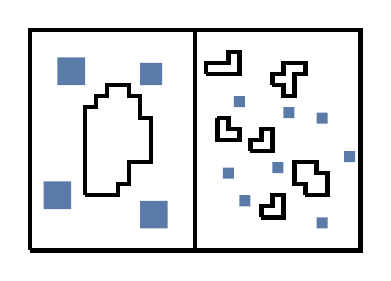
\begin{tikzpicture}[scale=0.7]
%\draw[help lines] (0,0) grid (6,4);

% Y1
\draw[ultra thick] (1,1) -- (1,2.6) -- (1.2,2.6) -- (1.2,2.8) -- (1.4,2.8) -- (1.4,3) -- (1.8,3) -- (1.8,2.8) -- (2,2.8) -- (2,2.4) -- (2.2,2.4) -- (2.2,1.6) -- (1.8,1.6) -- (1.8,1.2) -- (1.6,1.2) -- (1.6,1) -- (1,1);

% X1
% Blue: 88 122 160
\fill[fill=dblue!70] (0.5,3.5) -- (1,3.5) -- (1,3) -- (0.5,3) -- (0.5,3.5);
\fill[fill=dblue!70] (0.25, 0.75) -- (0.25, 1.25) -- (0.75,1.25) -- (0.75, 0.75) -- (0.25,0.75);
\fill[fill=dblue!70] (2,0.4) -- (2.5,0.4) -- (2.5,0.9) -- (2,0.9) -- (2,0.4);
\fill[fill=dblue!70] (2,3) -- (2,3.4) -- (2.4,3.4) -- (2.4,3) -- (2,3);

% Frame
\draw[ultra thick] (0,0) -- (3,0) -- (3,4) -- (0,4) -- (0,0);
\draw[ultra thick] (3,0) -- (6,0) -- (6,4) -- (3,4) -- (3,0);

% Y2
\draw[ultra thick] (3.2,3.2) -- (3.8,3.2) -- (3.8,3.4) -- (3.8,3.6) -- (3.6,3.6) -- (3.6,3.4) -- (3.2,3.4) -- (3.2,3.2);
\draw[ultra thick] (4,1.8) -- (4,2) -- (4.2,2) -- (4.2,2.2) -- (4.4,2.2) -- (4.4,1.8) -- (4,1.8);
\draw[ultra thick] (5,1) -- (5,1.2) -- (4.8,1.2) -- (4.8,1.6) -- (5.2,1.6) -- (5.2,1.4) -- (5.4,1.4) -- (5.4,1) -- (5,1);
\draw[ultra thick] (4.4,3) -- (4.4,3.2) -- (4.6,3.2) -- (4.6,3.4) -- (5,3.4) -- (5,3.2) -- (4.8,3.2) -- (4.8,2.8) -- (4.6,2.8) -- (4.6,3) -- (4.4,3);
\draw[ultra thick] (4.2,0.6) -- (4.2,0.8) -- (4.4,0.8) -- (4.4,1) -- (4.6,1) -- (4.6,0.6) -- (4.2,0.6);
\draw[ultra thick] (3.4,2.4) -- (3.6,2.4) -- (3.6,2.2) -- (3.8,2.2) -- (3.8,2) -- (3.4,2) -- (3.4,2.4);

% X2
\fill[fill=dblue!70] (3.8,0.8) -- (3.8,1) -- (4,1) -- (4,0.8) -- (3.8,0.8);
\fill[fill=dblue!70] (3.7, 2.6) -- (3.9,2.6) -- (3.9,2.8) -- (3.7,2.8) -- (3.7,2.6);
\fill[fill=dblue!70] (5.7, 1.6) -- (5.9,1.6) -- (5.9,1.8) -- (5.7,1.8) -- (5.7,1.6);
\fill[fill=dblue!70] (4.4,1.4) -- (4.4,1.6) -- (4.6,1.6) -- (4.6,1.4) -- (4.4,1.4);
\fill[fill=dblue!70] (3.5, 1.3) -- (3.7,1.3) -- (3.7,1.5) -- (3.5,1.5) -- (3.5,1.3);
\fill[fill=dblue!70] (5.2, 2.3) -- (5.4,2.3) -- (5.4,2.5) -- (5.2,2.5) -- (5.2,2.3);
\fill[fill=dblue!70] (4.6,2.4) -- (4.6,2.6) -- (4.8,2.6) -- (4.8,2.4) -- (4.6,2.4);
\fill[fill=dblue!70] (5.2,0.4) -- (5.4,0.4) -- (5.4,0.6) -- (5.2,0.6) -- (5.2,0.4);

\end{tikzpicture}
\end{center}

    \begin{itemize}
        \item How do we prove the discrete scale argument?
        %\pause

        \item Aside from $Z$'s dimension, we have little structural knowledge.
        %\pause

        \item Random choices of the $J_k$ avoid $Z$ effectively.

        %\pause
        \item We obtain for all but $o(1)$ of the length $L$ intervals in $I_k$, $J_k$ contains a length $L^\beta$ section of each, where $\beta = d(nd - \alpha)/(n - 1)$. This ratio gives the Hausdorff dimension bound $(nd-\alpha)/(n-1)$ for $X$.
    \end{itemize}
\end{frame}

\begin{frame}
    \frametitle{Conclusion}

    {\Huge So What's Next?}
\end{frame}

\begin{frame}
    \frametitle{Extension to Hausdorff Dimension}

    \begin{itemize}
        \item There is no obvious reason why our techniques should fail when $Z$ has {\it Hausdorff dimension} $\alpha$ rather than a Minkowski dimension bound.
        %\pause

        \item We are trying to use hyperdyadic coverings rather than coverings at a single scale to achieve this.
    \end{itemize}
\end{frame}

\begin{frame}
    \frametitle{Analogies with Hypergraphs}

    \begin{itemize}
        \item Partition $I_1, \dots, I_n$ into length $1/N^\beta$ sections. Form a hypergraph whose vertices are the sections, and add a hyperedge between $K_1 \subset I_1, \dots, K_n \subset I_n$ if $K_1 \times \dots \times K_n$ intersects $Z$.
        %\pause

        \item Our discrete configuration problem reduces to finding independant sets in hypergraphs.
        %\pause

        \item Many results in combinatorics have `sparse analogues' when generalized to hypergraphs and random techniques are used. In this work by thinking of dimension as a continuous analogue of `sparsity' we have come up with a continuous version of this.
        %\pause

        \item We are looking to using other methods on hypergraphs to improve the bound when $Z$ has certain structural properties.
    \end{itemize}
\end{frame}

\begin{frame}
    \frametitle{You're Interested in Learning More?}

Read these to find out more about configuration problems:

    \begin{itemize}
            \item Read Keleti (1999) for a simple use of scale discretization on a particular configuration avoidance problem.
            %\pause
            \item Read M\'{a}th\'{e} (2017) for a construction where $f$ is assumed to be a polynomial of bounded degree.
            %\pause
            \item Read Pramanik and Fraser (2018) for a general construction where $f$ is smooth and nonsingular. We generalize their work.
            %\pause
    \end{itemize}

    Thanks for listening!
\end{frame}

\end{document}